\documentclass{article}

\usepackage{graphicx}
\usepackage{tikz}
\usepackage{tikzsymbols}
\usetikzlibrary{calc,patterns,shapes.geometric}
\pagestyle{empty}
\usepackage[margin=0pt]{geometry}
\geometry{papersize={14in,12in}}

\def\centerarc[#1](#2)(#3:#4:#5){\draw[#1] ($(#2)+({#5*cos(#3)},{#5*sin(#3)})$) arc (#3:#4:#5);}

\begin{document}
	\begin{figure}
		\centering
		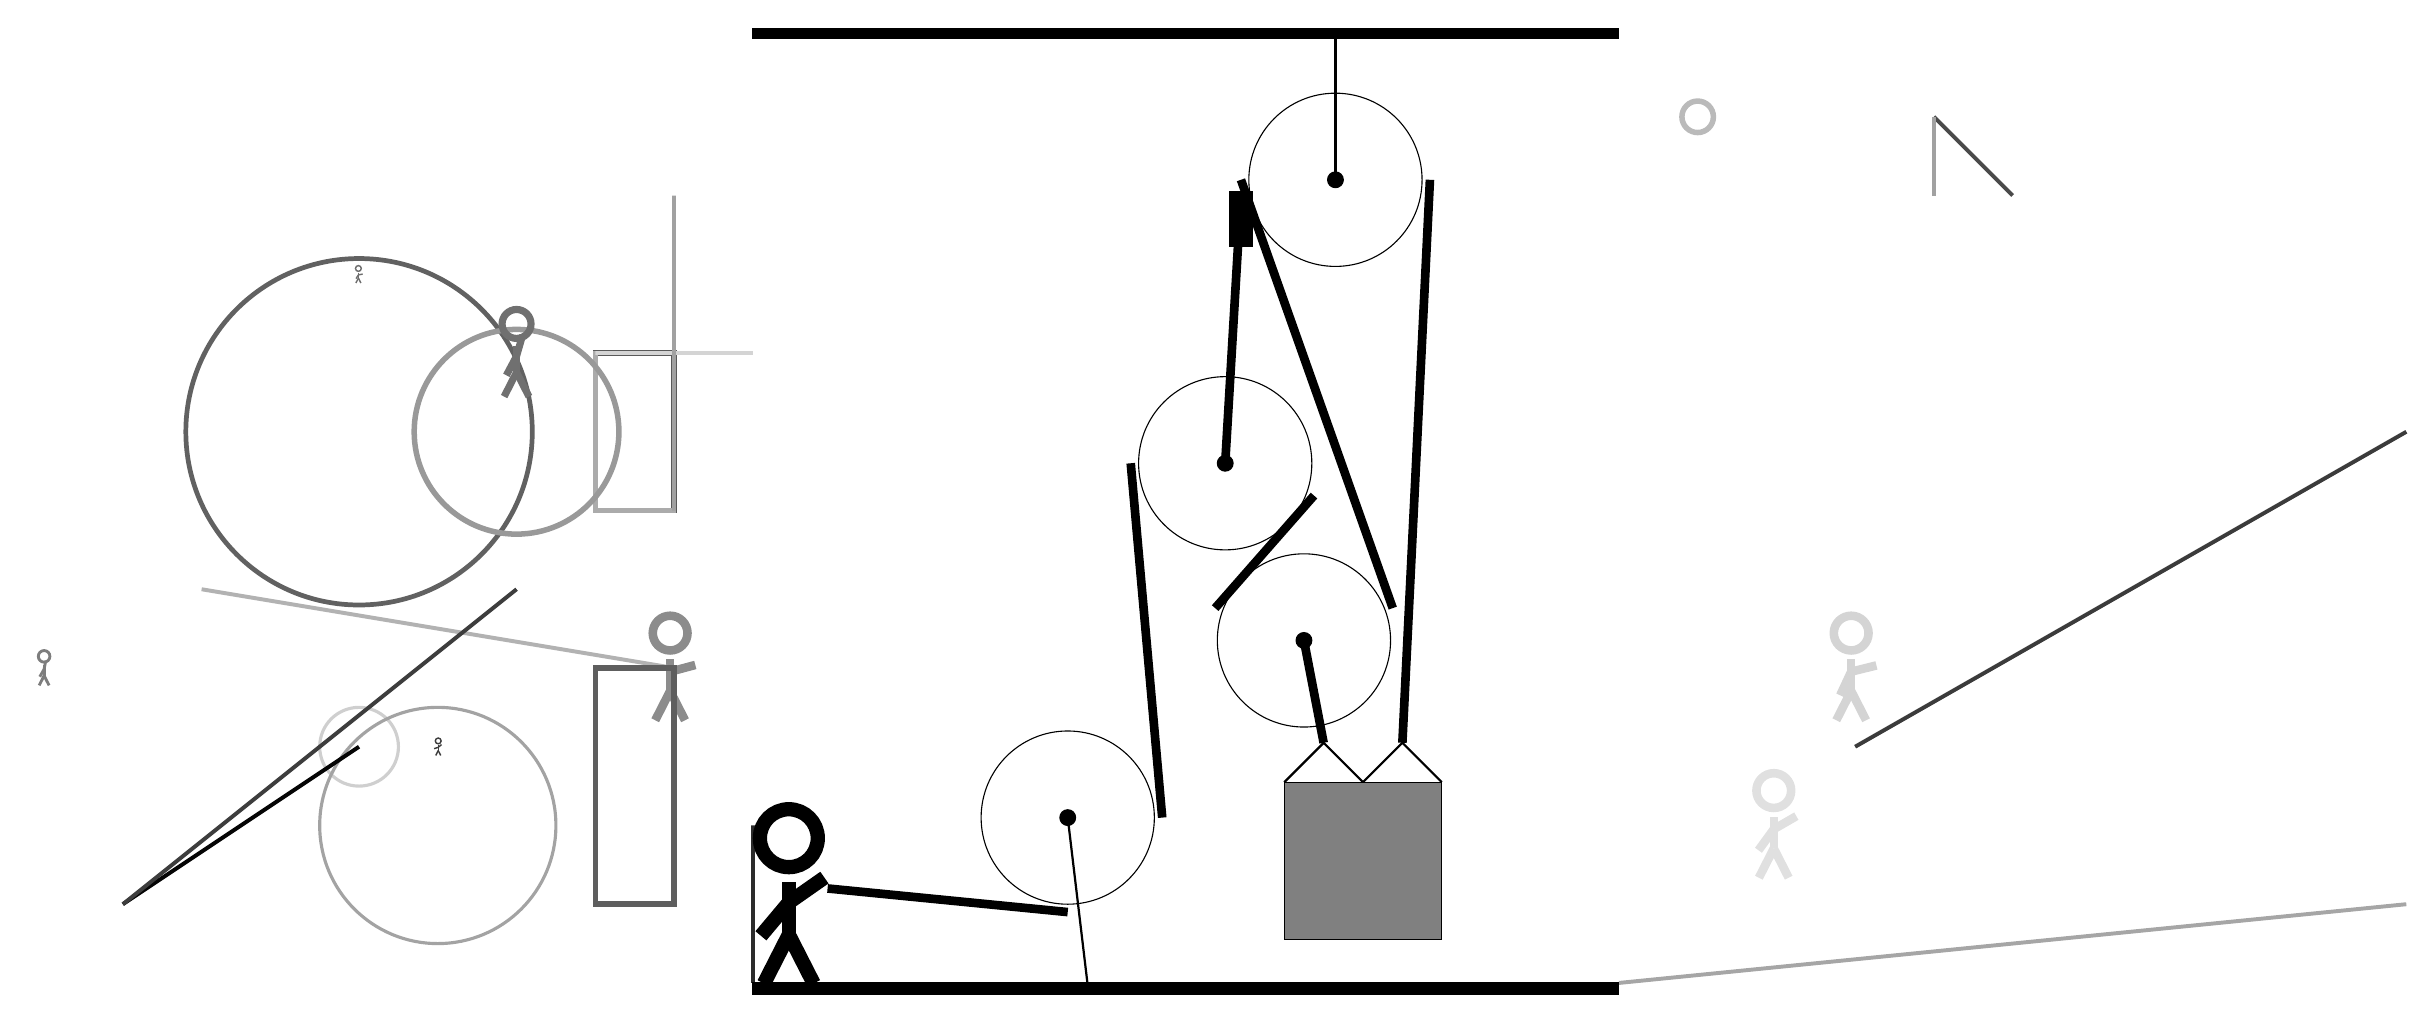
\begin{tikzpicture}
			%%%%% START %%%%%
			
			\draw[fill=black] (-6, 9) rectangle (5, 9.125);
			
			\draw (0, 3.6) circle (1.1);
			\draw[fill=black] (0, 3.6) circle (0.1);
			
			\draw (1, 1.35) circle (1.1);
			\draw[fill=black] (1, 1.35) circle (0.1);
			
			\draw[line width=0.7mm, color=black!65] (-7, 5) rectangle (-8, 3);
			
			\draw [line width=0.6mm, color=black!62](-11, 4) circle (2.2);
			\draw[line width=0.5mm, color=black!71](10, 7) -- (9, 8);
			\node[line width=0.6mm, color=black!57] at (-11, 6) {\Strichmaxerl[1][58][11]};
			
			\draw[line width=0.6mm, color=black!33] (-8, 3) rectangle (-7, 5);
			\node[line width=0.7mm, color=black!12] at (7, -1) {\Strichmaxerl[6][54][30]};
			\node[line width=0.7mm, color=black!45] at (-7, 1) {\Strichmaxerl[6][90][15]};
			\node[line width=0.2mm, color=black!17] at (8, 1) {\Strichmaxerl[6][65][14]};
			\draw[line width=0.4mm, color=black!17] (-8, 5) rectangle (-6, 5);
			
			\draw [line width=0.7mm, color=black!40](-9, 4) circle (1.3);
			\draw [line width=0.4mm, color=black!19](-11, 0) circle (0.5);
			\draw [line width=0.4mm, color=black!36](-10, -1) circle (1.5);
			\draw [line width=0.7mm, color=black!27](6, 8) circle (0.2);
			
			\node[line width=0.7mm, color=black!51] at (-15, 1) {\Strichmaxerl[2][60][79]};
			\node[line width=0.5mm, color=black!76] at (-10, 0) {\Strichmaxerl[1][18][40]};
			\draw[line width=0.5mm, color=black!98](-11, 0) -- (-14, -2);
			
			\node[line width=0.7mm, color=black!56] at (-9, 5) {\Strichmaxerl[5][62][74]};
			\draw[line width=0.5mm, color=black!37](9, 8) -- (9, 7);
			\draw[line width=0.6mm, color=black!37] (-7, 7) rectangle (-7, 3);
			\draw[line width=0.5mm, color=black!30](-7, 1) -- (-13, 2);
			\draw[line width=0.5mm, color=black!83] (-6, -1) rectangle (-6, -3);
			\draw[line width=0.5mm, color=black!76](-9, 2) -- (-14, -2);
			\draw[line width=0.5mm, color=black!77](8, 0) -- (15, 4);
			\draw[line width=0.5mm, color=black!35](5, -3) -- (15, -2);
			\draw[line width=0.7mm, color=black!63] (-8, -2) rectangle (-7, 1);
			
			
			\draw (1.4, 7.2) circle (1.1);
			\draw[fill=black] (1.4, 7.2) circle (0.1);
			\draw[very thick] (1.4, 7.2) -- (1.4, 9);
			
			\draw (-2, -0.9) circle (1.1);
			\draw[fill=black] (-2, -0.9) circle (0.1);
			\draw[thick] (-2, -0.9) -- (-1.75, -3);
			
			
			\draw[thick]  (0.75, -0.45) -- (1.25, 0.05) -- (1.75, -0.45) -- (2.25, 0.05) -- (2.75, -0.45);
			\draw[fill=black!50] (0.75, -0.45) rectangle (2.75, -2.45);
			\draw[line width=1.1mm] (-5.05, -1.8) -- (-2, -2.1);
			\centerarc[line width=1.1mm](-2, -0.9)(270:360:1.2000000000000002);
			\draw[line width=1.1mm] (-0.8, -0.9) -- (-1.2, 3.6);
			\draw[line width=1.1mm] (0, 3.6) -- (0.2, 7.0);
			\draw[line width=1.1mm, fill=black](0.1, 6.4) rectangle (0.3, 7.0);
			\centerarc[line width=1.1mm](0, 3.6)(-20:180:1.2000000000000002);
			\draw[line width=1.1mm] (1.1276, 3.1896) -- (-0.1276, 1.7604);
			\centerarc[line width=1.1mm](1, 1.35)(160:380:1.2000000000000002);
			\draw[line width=1.1mm] (2.1276, 1.7604) -- (0.2, 7.2);
			\draw[line width=1.1mm](1, 1.35) -- (1.25, 0.05);
			\centerarc[line width=1.1mm](1.4, 7.2)(0:180:1.2000000000000002);
			\draw[line width=1.1mm] (2.6, 7.2) -- (2.25, 0.05);
			
			\node at (-5.5, -1.9) {\Strichmaxerl[10][50][35]};
			
			\draw[fill=black] (-6, -3) rectangle (5, -3.15);
			
			%%%%% END %%%%%
		\end{tikzpicture}
	\end{figure}	
\end{document}